%%% template.tex
%%%
%%% This LaTeX source document can be used as the basis for your technical
%%% paper or abstract. Intentionally stripped of annotation, the parameters
%%% and commands should be adjusted for your particular paper - title, 
%%% author, article DOI, etc.
%%% The accompanying ``template.annotated.tex'' provides copious annotation
%%% for the commands and parameters found in the source document. (The code
%%% is identical in ``template.tex'' and ``template.annotated.tex.'')

\documentclass[review]{acmsiggraph}

\usepackage{subcaption}
\usepackage[]{algorithm2e}


\usepackage[usenames,dvipsnames]{color}
\newcommand\memo[1]{{\color{CornflowerBlue}#1}}
\newcommand\devin[1]{{\color{BurntOrange}#1}}
\newcommand\julien[1]{{\color{RubineRed}#1}}
\newcommand\claudia[1]{{\color{Purple}#1}}
\newcommand\panayiotis[1]{{\color{Green}#1}}
\newcommand\note[1]{{\color{Red}#1}}

\newcommand{\etal}{et al.\xspace}

\usepackage{amsfonts}
\usepackage{amssymb}
\usepackage{graphicx}
\usepackage{url}
%\usepackage[tight,footnotesize]{subfigure}
%\usepackage{algorithm}
%\usepackage{algorithmic}


\TOGonlineid{45678}
\TOGvolume{0}
\TOGnumber{0}
\TOGarticleDOI{1111111.2222222}
\TOGprojectURL{}
\TOGvideoURL{}
\TOGdataURL{}
\TOGcodeURL{}

\title{Optimization-based computation of locomotion trajectories for Crowd Patches}

\author{Authors\thanks{e-mail:emails@emailplace}\\Institution}
\pdfauthor{Authors}

\keywords{keywords go here}

\begin{document}

%% \teaser{
%%   \includegraphics[height=1.5in]{images/sampleteaser}
%%   \caption{Spring Training 2009, Peoria, AZ.}
%% }

\maketitle

\begin{abstract}

For many years now, simulating crowds in virtual environments have become more and more important. We want to see crowds in movies, TV shows, video-games, etc, and we want them to look good and natural.  An important part of crowd simulation is the way the people (or animals or any other moving agent inhabiting the environment) walk from one place to another. This paper concentrates in improving the crowd patches approach suggested by Yersin et al. ~\cite{Yersin:2009}. This method is based on the construction of animation blocks (called patches) stuck together to create a bigger and richer animation. The main purpose of this paper is to improve the way trajectories are created using an optimization-based method. Our main contributions include a better way to match the end points of trajectories using the Gale-Shapley algorithm~\cite{gale1962college} , a better method for collision avoidance that allows a more natural look to trajectories, as well as a proposal for smoothing the final trajectories using cubic splines. We show in the results several examples of patches and how they were improved by our method. We also discuss limitations and future work in the final sections.



%Citations can be done this way~\cite{Jobs95} or this more concise way~\shortcite{Jobs95}, depending upon the application.

\end{abstract}

\begin{CRcatlist}
%  \CRcat{I.3.3}{Computer Graphics}{Three-Dimensional Graphics and Realism}{Display Algorithms}
  %\CRcat{I.3.7}{Computer Graphics}{Three-Dimensional Graphics and Realism}{Radiosity};
\end{CRcatlist}

\keywordlist

%% Use this only if you're preparing a technical paper to be published in the 
%% ACM 'Transactions on Graphics' journal.

\TOGlinkslist

%% Required for all content. 

\copyrightspace

\section{Introduction}
\label{sec:intro}

Video Games are constantly displaying larger and livelier virtual environments due to increased computational power and advanced rendering techniques.
For example, the recent Grand Theft Auto (GTA) game~\cite{GTA:web} takes place in Los Santos and its surroundings, a completely virtual city.
In spite of the impressive quality and liveliness of the scene, Los Santos still remains relatively sparsely populated with virtual people.
The reason for this phenomenon is the large computational cost required to get an {\it ambient crowd} in such large environments.
To address this issue, the technique of {\it Crowd Patches} has been recently introduced by Yersin \etal \cite{Yersin:2009}.

{\it Crowd patches} are precomputed elements (patches) of crowd animations.
Patches are time-periodic so that they can be endlessly played in time.
The boundary conditions of precomputed animations are accurately controlled to enable combining patches in space (i.e., characters can move from in-between patches) and compose large ambient crowds.
This technique eases the process of designing performance efficient ambient crowds. 

One problem with this technique however, is the computation of internal animation trajectories for patches that satisfy both, time-periodicity and boundary conditions amongst patches.
Satisfying both of these constraints is difficult, since it is equivalent to computing collision-free trajectories that exactly pass through spatio-temporal waypoints (i.e., at some exact position in time) whilst at the same time solving possibly complex interactions between agents (collision-avoidance).
In addition to that, trajectories should look as natural as possible.

In this paper we propose a new optimization-based method to compute these internal trajectories.
Our method starts by initially assigning linear space-time trajectories which are easy to compute and satisfy both, periodicity and boundary conditions, but at the same time might introduce collisions between characters.
Then, iteratively, we optimize the trajectories to handle collisions.
We try to keep the generated trajectories as close as possible to the initial linear trajectories, to minimize the magnitude of collision-avoidance maneuvers.
\panayiotis{How do we define this? Do we measure it?}
\panayiotis{Could we present this as the principle of \textbf{least effort}; i.e. the agents do as little as possible to achieve their goals without doing any complex movement\ldots}

To conclude, the main contribution of this work is an optimization-based algorithm to compute high quality animation trajectories ($2D$ global navigation trajectories) for individual crowd patches under constraints (expressed as a set of spatio-temporal boundary control points).

The remainder of this paper is organized as follows: Section \ref{sec:star} proposes a short overview on the state of the art. Section \ref{sec:method} details our technique to compute these internal trajectories. Then, in Section \ref{sec:results} some results, together with their performance and quality analysis are shown before a brief discussion and concluding remarks (Sections~\ref{sec:discussion} and \ref{sec:conclusions} respectively). 

\section{State of the Art}
\label{sec:star}

Most often, virtual environments are populated based on crowd simulation approaches~\cite{ThalmannBook:2013}.
An ambient crowd is generated from a large set of moving characters, mainly walking ones.
Recent efforts in crowd simulation have enabled dealing with improving computational performance~\cite{PettreCAVW:2006,Treuille:2006}, dealing with high densities~\cite{Narain:2009} or controllable crowds~\cite{Guy:2009}.
There has also been a lot of effort to develop velocity-based approaches~\cite{Paris:2007,VanDenBerg:2008} which display much smoother and realistic locomotion trajectories, especially thanks to anticipatory adaptation to avoid collisions between characters.

Simulation-based techniques seem ideal for creating an ambient crowd for large environments but several problems are recurrent with such approaches:
a) crowd simulation is computationally demanding, crowd size is severely limited for interactive applications on light computers;
b) simulation is based on simplistic behaviours (e.g., walking, avoiding collisions, etc.) and therefore it is difficult to generate diverse and rich crowds based on classical approaches;
c) crowd simulation is prone to animation artifacts or deadlock situations and it is thus impossible to guarantee animation quality. 

Example-based approaches attempt to solve the limitations on animation quality.
The key idea of this approaches is to indirectly define the crowd behavior rules from existing crowd data (such as trajectories from real people)~\cite{Lerner:2007,Ju:2010,Charalambous:2014}.
Locally, trajectories are typically of good quality, because they reproduce real recorded ones.
However, such approaches raise other difficulties: it is difficult to guarantee that the example database will cover all the required content and it can also be difficult to control behaviors and interactions displayed by characters if the database content is not carefully selected.
Finally, those approaches are most of the time computationally demanding; even more so than traditional simulation based techniques.

To solve both performance as well as quality issues, crowd patches were introduced by Yersin \etal~\cite{Yersin:2009}.
The key idea is to generate an ambient moving crowd from a set of interconnected patches.
Each patch is a kind of $3D$ animated texture element, which records the trajectories of several moving characters.
Trajectories are periodic in time so that the crowd motion can be played endlessly.
Trajectories' boundary conditions at the geometrical limits of patches are controlled to be able to connect together two different patches with characters moving from one patch to another.
Thus, a crowd animated from a set of patches have a seamless motion and patches' limits cannot easily be detected.
The boundary conditions are all registered into {\it patterns}, which are sort of gates for patches with a set of spacetime input/output points.
%For a more detailed expanation on the crowd patches approach please refer to~\cite{Yersin:2009}. 

Nevertheless, using the crowd patches approach, a limited set of patterns should be used to be able to connect various patches together.
% Therefore, instead of defining patches directly; these can be indirectly defined from a set of patter
As a result, it is important to be able to compose a patch by starting from a set of patterns, and then deducing internal trajectories of patches from the set of boundary conditions defined by the patterns.
As a result, we need to compute trajectories for characters that pass through a given set of spatio-temporal waypoints; i.e., characters should reach specific points in space at specific moments in time.
This problem is difficult since generally speaking steering techniques for characters consider $2D$ spatial goals, but do not consider the time a character should take to reach its waypoint.
Therefore, dedicated techniques are required. 

Yersin~\etal suggest using an adapted Social Forces technique to compute internal trajectories~\cite{Helbing:2005}.
The key idea is to connect input/output points together with linear trajectories and model characters as particles attracted by a goal moving along one of these linear trajectories, combined with repulsion forces to avoid collision between them and static obstacles.
One problem with this approach is limited density level, as well as the level of quality of trajectories that suffer from the usual drawbacks of the Social Forces approach such as lack of anticipation, which results into unnatural looking local avoidance maneuvers (Figure~\ref{fig:res:helbing}).

Compared to previous techniques we suggest formulating the problem of computing internal trajectories as an optimization problem.
First, we suggest optimizing the way input and output points are connected.
Especially, since waypoints are defined in space and time, we connect them aiming for {\it comfortable} walking speeds (i.e., close to the average human walking speed).
Indeed, characters moving too slow or too fast are visually evident artifacts.
Secondly, after having connected waypoints with linear trajectories, we deform them to remove any collisions by employing an iterative approach.
This approach aims at minimizing the changes to the initial trajectories.
%We do this through an iterative process trying to remove collisions with as limited as possible changes to the initial trajectories.
We demonstrate improvements in the quality of results as compared to the original work by Yersin \etal (Figure~\ref{fig:res:helbing}).



\section{Methodology}
\label{sec:method}

%%----------------------------------------------------------------
%% Overview Figure
%%----------------------------------------------------------------
\begin{figure*}[t]
	\begin{center}
	
\includegraphics[width=0.9\linewidth]{./images/overview-hd.png}
% 	\includegraphics[height=4cm]{./images/patches-empty-patch-with-pattern.png}
% 	\includegraphics[height=4cm]{./images/patches-connected-patch.png}
% 	\includegraphics[height=4cm]{./images/patches-collision-free-patch.png}
% 	\includegraphics[height=4cm]{./images/patches-smoothed-patch.png}
	\caption{
		\textbf{Overview} Input and output points in a patch's patterns are initially connected and subsequently modified using the proposed optimization approach and smoothed out to be collision free.
	}
	\label{fig:overview}
	\end{center}
\end{figure*}
%%----------------------------------------------------------------
%% Overview Figure
%%----------------------------------------------------------------

\note{Overview: remind definitions on crowd patches: patch, pattern, spatiotemporal waypoints (boundary conditions: input, output, initial states // boundary conditions should be strictly enforced. Movable control points), period of time \dots}

In this section we present the proposed methodology for generating trajectories for patches.
We first give some definitions and notations (Section~\ref{sec:method:definitions}), followed by an overview of the method (Section~\ref{sec:method:overview}), and trajectories initial generation, collision handling and smoothing out (Sections~\ref{sec:method:init}--\ref{sec:method:smoothing}).


\note{Starting Definitions:}
\subsection{Definitions}
\label{sec:method:definitions}

Before presenting our approach on trajectory generation for Crowd Patches, we present some definitions regarding Crowd Patches as presented by Yersin \etal~\cite{Yersin:2009}.
 
 
\begin{description}

\item[Patch]{
A patch is a set $\{ A, \pi, D, S\}$ where $A$ is a geometrical area with a convex polygonal shape, $\pi$ the period of time of the animation and $D$ and $S$ are the sets of dynamic and static objects, respectively.
These last two sets may be empty in case of an empty patch.
}

\item[Static obstacles]{
Static objects are simple obstacles whose geometry is fully contained inside the patch.
}

\item[Dynamic objects]{
Dynamic objects are animated; i.e., they are moving in time according to a set of trajectories $T$.
}

\end{description}

We define a {\bf trajectory} inside a patch as a function $\tau$ going from time to position, more specifically from a subset of $[ 0,\pi ]$ to $A$.

$ \tau:[t_1,t_2]\rightarrow A, \hspace{0.3cm} 0 \leq t_1 < t_2 \leq \pi$.
We represent a trajectory as a list of control points connected by segments. 
\note{THIS I A LITTLE BIT CONFUSING}

A {\bf control point} is a point in space and time $\mathbf{cp} = \{\mathbf{p}_{cp}, t_{cp}\}$. All control points in a trajectory can either be boundary or movable ones. Boundary control points serve as entry and exit points to the patch and cannot be moved, added or deleted. Movable control points can be moved, added, or removed from the trajectory as long as they do not violate the constraints of the patch; i.e., their positions $\mathbf{p}_{cp}$ must lie inside area $A$ and their time $t_{cp}$ must be between $t_1$ and $t_2$.

A {\bf segment} is a straight line connecting two control points in a specific order. Since these are unidirectional lines in space-time, it is important to remember that they are not allowed to go backwards in time.

There are two categories of dynamic objects: endogenous and exogenous agents. {\bf Endogenous agents} remain inside $A$ for the total period of time $\pi$. In order to achieve periodicity for the animation, they are associated with a trajectory $\tau : [0,\pi] \rightarrow A$, such that it respects the periodicity condition: the position at the start and at the end of the animation must be the same, i.e. \mbox{$\tau (0) = \tau (\pi)$}.\\
{\bf Exogenous agents} go outside $A$. They enter the patch at time $t_{initial}$ and position $\mathbf{p}_{initial}$, and they exit at time $t_{final}$ and position $\mathbf{p}_{final}$. For each agent we associate a sequence of $n \ge 1$ trajectories $\{ \tau_1, \tau_2, \dots, \tau_n\}$. Sequences may have only one trajectory, but some agents require additional trajectories in order to satisfy speed and time constraints. The following conditions must be respected in each sequence of trajectories associated with an exogenous agent:

\begin{itemize}

\item{$\mathbf{p}_{initial}$ and $\mathbf{p}_{final}$ must be points in the border of $A$. Otherwise, they couldn't be exogenous agents.}

\item{If the sequence is composed by more than one trajectory, for each two contiguous trajectories, the following must be true to ensure continuity: $\tau_i(\pi) = \tau_{i+1}(0)$.}

\end{itemize}

Note that the second condition implicitly implies that in sequences with multiple trajectories, each middle trajectory must be fully defined in the period of time $[0,\pi]$, while $\tau_1$ must be defined in $[t_{initial},\pi]$ and $\tau_n$ must be defined in $[0, t_{final}]$.

\begin{description}

\item[Pattern -]{If a patch is a spatio-temporal cube (or any other right prism, depending on the type of polygon used as its area, then a pattern could be defined as one lateral side of the \note{cube (or right prism).} Specifically, it is a rectangle whose base is one of the edges of the polygonal area (we define \boldmath{${l}$} as this two dimensional vector), and its height is equal to the period $\pi$. These patterns also include the sets of boundary control points. We divide this set evenly into two subsets: Input and Output. The Input set contains the boundary control points where exogenous agents begin their trajectories; we call these Entry Points. Conversely the elements of Output are called Exit Points. They establish the position in time and space that the exogenous agents finish their paths. Formally defined, a patch P is:
$$ P = \{l, \pi, I_i [p_i, t_i], O_j[p_j, t_j]\}$$
We populate virtual environments by sticking patches together. Thus, we have to ensure continuity between trajectories for exogenous agents passing through two contiguous patches. This means that two adjacent patches must \note{have a similar pattern on the side they share}. The vector $l$ and period $\pi$ must be equivalent and the sets of Input and Output are exchanged. If we have $P_1=\{\mathbf{l}, \pi, I [p_1,t_1], O[p_2,t_2]\}$ and $P_2=\{\mathbf{l'}, \pi', I'[p'_2, t'_2], O'[p'_1, t'_1]\}$, then, in order to satisfy $C^0$ continuity we must ensure: 
$$ l=l', \pi=\pi', p_1=p'_1, t_1=t'_1, p_2=p'_2, t_2=t'_2.$$
We then say $P_1$ is the mirror pattern of $P_2$. In the animation, this will be seen as an agent going from one patch to an adjacent one. 
If the area of a patch is a square, the patch defines 4 patterns, one for each of its sides. Patterns defined by a patch have the property that the sum of the cardinality of all the Inputs is the same as the sum of the cardinality of all Outputs. We call this the parity condition: $\sum(|Inputs|)= \sum(|Outputs|)$.

A patch defines a set of Patterns, and conversely, a set of patterns satisfying the parity condition, having the same period, and whose vectors define a convex polygonal area, can be used to create a patch. 
 }

\end{description}

\subsection{Overview}
\label{sec:method:overview}

The objective is, given a set of patterns, we want to construct a patch.
This process has three main steps:
\begin{enumerate}
  \item Make a matching between the elements in the Input and Output sets contained within a patch. In this step, we connect Entry to Exit Points based on a scoring function. This function tries to keep agents close to their prefered speed while at the same time avoiding connections to similar patterns, thus reducing unwanted u-turns.  The input for this function is a set of patterns and the output is a set of piecewise linear trajectories connecting the entry and exit points.
  \item Create collision free trajectories for these pairings. We start with simple line trajectories and start bending them until they are collision free. Points lying at the borders, i.e. the Entry and Exit points, are hard restraints and can never be moved.
  \item Smoothing trajectories (if needed).  Last, we use splines to minimize the hard turns. We make sure the new trajectories stay close to the original ones, lest we create new collisions.
\end{enumerate}

\note{Problem : is to compute internal trajectories that join all boundary conditions with conitnuous and believable motion trajectories. 

2 steps: 
 - step 1: connect waypoints
INPUT first boudnary conditions are ``alone'' in patches $\rightarrow$ associate/connect waypoints
 them 
OUTPUT : initial trajectories (piecewise linear trajs, possibly colliding, with ``good'' properties that we will define later on)

 - step 2: optimize intial trajectories by moving control points to remove collisions
    INPUIT : initial trazjectories
      OUTPUT : colliision trajectories, still enforcing boundary conditions
      
- step 3 is smoothing
}       


\subsection{Connecting Boundary Control Points}
\label{sec:method:init}

The first step to this algorithm is to match all the entry and exit points.  To do this, we have to measure how good or bad a match is. Intuitively, there are some better matches than others, Judging by sight, trajectories passing near the center of the patch look better that the ones staying close to the borders. We can consider some other aspects too, like how close the speed needed for the agent to go from the Entry Point to the Exit Point is to comfort speed. We use a comfort speed $u_{cft}$ of $1.33~m/s$ which is the normal walking speed of humans in an unconstrained environment.

For a square patch, we prefer to match points with points on the opposite pattern. Then the points on the contiguous pattern and finally, the points that are in the same pattern. If there are multiple options on the same pattern we choose the point whose associated trajectory is closest to comfort speed.

To solve this matching problem, we make use of the Gale-Shapley algorithm~\cite{gale1962college} (see Algorithm~\ref{alg:stable-matching}), commonly referred to as the algorithm to solve the stable marriage problem.  This algorithm assures that at the end, if we have Alice engaged to Bob and Carol engaged to Dave, it is not possible for Alice to prefer Dave and Dave to prefer Alice. We call that a stable matching.  

This pseudocode demonstrates the Gale-Shapley algorithm in relation to two equal lists of men and women who are being matched for marriage. However the algorithm generalizes to any matchable objects, which in our case is entry and exit points.

%%-------------------------------------------------------------------
%% The Stable Matching Algorithm by Gale-Shapley
%%-------------------------------------------------------------------
\begin{algorithm}[t]

Initialize all $m \in M$ and $w \in W$ to \textit{free} \;
\While {$ \mathbf{\exists}$ \textit{free} man $m$ who still has a woman $w$ to propose to} {
	$w \leftarrow m's$ highest ranked woman to whom he has not yet proposed \;
	\eIf {$w$ is \textit{free}}
	{ 
		$(m,w)$ become engaged \;
	}
	{
		some pair $(m',w)$ already exists \;
		\eIf {$w$ prefers $m$ to $m'$} 
		{
			$(m,w)$ become engaged \;
			$m'$ becomes \textit{free} \;
		}
		{
			 $(m',w)$ remain engaged;
		}
	}
}
\caption{Stable Matching Algorithm}
\label{alg:stable-matching}
\end{algorithm}
%%-------------------------------------------------------------------
%% The Stable Matching Algorithm by Gale-Shapley
%%-------------------------------------------------------------------


All we need in order to use this algorithm is a to generate preferences for entry and exit points. We do this with the following steps:
\begin{enumerate}
  \item Find the speed it would take to travel from an Entry Point to an Exit Point.  Letӳ assume $(\mathbf{p}_1, t_1)$ is position and time of the Entry Point and $(\mathbf{p}_2,t_2)$ the equivalent of the Exit point. Speed $u$ is $d/t$ where $d=|\mathbf{p}_1-\mathbf{p}_2|$ and $t=t_2-t_1$ in case $t_2>t_1$. Otherwise, $t=period+t_2-t_1$. More details on why we take this time will be given later when we create the initial set of trajectories.
  \item Now, we assign each pair of points a number between $0$ and $\pi/2$, where $0$ represents maximum closeness to comfort speed with $arctan(|u_{cft} -u|)$.
  \item We add penalties for points being in the same patch, for those points, we add $4$. For points lying in the contiguous pattern we also add a smaller penalty, $2$.
  \item We sort each list.
\end{enumerate}
\panayiotis{The steps above need editing}    
 
We will have a list similar to this for each entry and exit point, we call this list the proposal list (see Table ~\ref{tab:proposal-list}).

%%-------------------------------------------------------------------
%% The Proposal List table
%%-------------------------------------------------------------------
\begin{table}[b]
	\centering
	\caption{Proposal List}
	\begin{tabular}{|c|c|}
		\multicolumn{2}{c}{Rankings of preferred}\\
		\multicolumn{2}{c}{partners for Entry Point A}\\
		\hline
		Preference	& Exit Point\\
		\hline\hline
		$0.34$		&	B\\
		$1.3$		&	C\\
		$2.3$		&	A\\
		$2.4$		&	E\\
		$4.5$		&	D\\
		$4.6$		&	F\\
		\hline
		\end{tabular}
	\label{tab:proposal-list}
\end{table}
%%-------------------------------------------------------------------
%% The Proposal List table
%%-------------------------------------------------------------------


Exit Points F and D lie in the same pattern as Entry Point A, so they receive a higher number.
After this, we use the stable matching algorithm mentioned above.

Every two points that remained engaged at the end of the algorithm become a pair.
The last step is to create the initial batch of trajectories. We start by trying to connect the points with a straight line. We do something special when a line tries to travel backwards in time, i.e. $t_2<t_1$. For these cases we split the initial trajectory in two. One going from $t_1$ to period $\pi$, another one going from $0$ to $t_2$.  The positions of these new control points are in the same straight line, taken in such a way that the speed is the same going from $t_1$ to $\pi$ and from $0$ to $t_2$. We use the same method if the trajectory is moving at unrealistically fast speeds.

We make further adjustments in the initial trajectory in some special cases. For agents traveling only over the edge, we add a control point near the center of the patch. For agents moving slowly we add a control point with same position, but different time, thus making the agent do a full stop (as if pausing to look around), after a few moments it continues its journey with a better speed.

\devin{The output of this function is a set of trajectories. Collisions are probably still present in the trajectories at this point.}
 

\note{
- INPUT OUTPUT objective

- when you connect two boundary conditions, you connect two spation temporal waypoints. This means that you determine this way where characters enter, where they exit patches and the speed between waypoints. 

- we can define what is a ԧoodԠconnection: avoid half turn, avoid extreme speeds. 

- we define an objective function, we solve this using the stable marriage problem. 

- reminder of 2009 paper - you explain the specific case of splitting trajectories. 

-  you provide pseudo algo for this,  

 - you define all the variables/parameters you use. 
 
summarize what you get as an aoutput, and what is the next step.
}



\subsection{Removing Collisions}
\label{sec:method:remove-collisions}

\panayiotis{Make sure for all the equation that the correct symbols are inserted: bold for vectors, normal fonts for scalars, etc.}

We are given a set of trajectories within a patch consisting of both movable and boundary control points. What we expect in return is modified trajectories that have maintained their spatio-temporal entrance and exit points while removing all collisions throughout the entire period of the patch. Our objective is to use these patches in larger crowd simulations of people. We would like to create trajectories that could represent human motion. We focus on creating collision free motion since obvious collisions in simulations greatly reduces the realism of the animation.





Given two trajectories you can find the distance between them at any moment in time. The shortest distance between trajectories is the minimum of all these distances computed over the period of the patch. To compute the minimum distance between two trajectories we find the minimum distance between all the segments of the trajectories and take the minimum of the minimums as our final answer. When looking at two segments we find the intersection of the time intervals. If the intersection is not empty, we find the minimum distance. We call the start and end time of this intersection $t_0$ and $t_1$ respectively.

Each one of those segments represent a moving agent with an initial position $\mathbf{p}_0$ and $\mathbf{p}_1$ with velocities $\mathbf{v}_0$ and $\mathbf{v}_1$ moving in the time interval $[t_0,t_1]$. 

We can then define the distance at a certain time between the two segments with the following equation.

\begin{equation}
	d(t) = || (\mathbf{p}_0+\mathbf{v}_0*t) - (\mathbf{p}_1+\mathbf{v}_1*t) ||
	\label{eqn:distance}
\end{equation}

For simplicity we say $ \mathbf{w} = \mathbf{p}_0-\mathbf{p}_1$ and $\mathbf{dv} = \mathbf{v}_0-\mathbf{v}_1$, so then,

\begin{equation}
	d(t) = || \mathbf{w} + \mathbf{dv}*t ||
	\label{eqn:distance_simple}
\end{equation}



We are looking for the minimum so we solve for $t$ when when the derivative equals zero.
\begin{equation}
	t_c = (-\mathbf{w} \cdot \mathbf{dv}) / || \mathbf{dv} ||^2
\end{equation}

With $t_c$, the time at which the two line segments are closest we can easily calculate the position on each of those segments, and thus the distance between them. If the time is outside the bounds of the segment we check the endpoints of the line segment for collision.


%%-------------------------------------------------------------------
%% Removing collisions figure
%%-------------------------------------------------------------------
\begin{figure*}[t]
	\begin{center}
	\includegraphics[width=0.3\linewidth]{./images/collision-2D-example-with-collision.png}
	\includegraphics[width=0.3\linewidth]{./images/collision-2D-example-without-collision.png}
	\includegraphics[width=0.3\linewidth]{./images/collision-2D-example-overlay.png}
	\\
	\includegraphics[width=0.3\linewidth]{./images/key-entry-exit-point.png}
	\caption{
		\textbf{\textbf{Collision removal}}
	}
	\label{fig:collision-removal}
	\end{center}
\end{figure*}
%%-------------------------------------------------------------------
%% Removing collisions figure
%%-------------------------------------------------------------------




We compute a minimum distance between each pair of trajectories. We store each value in a minimum distance matrix $M$. The position in the matrix corresponds to the trajectory ID. So the value at $M(i, j)$ would be the minimum distance from trajectory $\tau_i$ to trajectory $\tau_j$. It's good to note that this value will be the same as $M(j,i)$. Furthermore $M(i,i)$ will always be zero and distance for trajectories that don't intersect in time, we set them to a number bigger than the threshold for collisions, for example $100$ for a threshold of $1$ (see Table ~\ref{tab:minimum-distances}). These facts can be used to reduce computation while filling out the minimum distance matrix.

%%-------------------------------------------------------------------
%% The Minimum Distances Table
%%-------------------------------------------------------------------
\begin{table}[t]
	\centering
	\caption{Minimum Distances}
	\begin{tabular}{|c||c|c|c|}
		\hline
		 & $\tau_0$	& $\tau_1$ & $\tau_2$\\ \hline \hline
		$\tau_0$	& $0$		&	$100$ & $8.31$\\  \hline
		$\tau_1$	& $100$		&	$0$ & $0.14$\\  \hline
		$\tau_2$	& $8.31$		&	$0.14$ & $0$\\
		\hline
		\end{tabular}
\label{tab:minimum-distances}
\end{table}
%%-------------------------------------------------------------------
%% The Proposal List table
%%-------------------------------------------------------------------

\panayiotis{Do we have an image for this distance matrix?}
\memo{Actual image? Or a table? I can do that anyways, as soon as I figure out how to create a nxn table in latex}

Our algorithm (see Algorithm~\ref{algo:control-points}) creates collision free trajectories by adding and modifying control points. We can guarantee this by looking at the minimum distance matrix. If every value in the matrix is above some threshold then we know that for the entire period of the patch no two agents come closer than that threshold. So if we make that threshold equal to the sum of the radii being compared, those agents will never touch.

\panayiotis{Write the pseudo code in an algorithm format}

%%-------------------------------------------------------------------
%% Control Points algorithm
%%-------------------------------------------------------------------
\begin{algorithm}[t]
Compute minimum distance matrix $M$\;
\While{there exists at least one entry in $M$ below the threshold}{
	Find indices $i$  and $j$ for which $M(i,j)$ has the smallest value $d$\;
	Create temporary control points $\mathbf{cp}_i$ and $\mathbf{cp}_j$ in $\tau_i$ and $\tau_j$ that are at distance $d$ \;
	Apply repulsion forces to $\mathbf{cp}_i$ and $\mathbf{cp}_j$\;
	Update  $\tau_i$ and $\tau_j$\;
	Update $M$ \;
	}
\caption{The control points generation algorithm}
\label{algo:control-points}
\end{algorithm}
%%-------------------------------------------------------------------
%% Control Points algorithm
%%-------------------------------------------------------------------


We begin by computing the minimum distance matrix. Then while collisions still exist we find the smallest value in the minimum distance matrix. From that we find the corresponding trajectories and a point of closest approach for each trajectory $\mathbf{p}_1$ and $\mathbf{p}_2$. We then find an updated position for each of these points.

To find the the updated position of a new point we add a correction force $\mathbf{F}_c$ to its current position $\mathbf{p}_1^{old}$.


\begin{equation}
	\mathbf{p}_1^{new} = \mathbf{p}_1^{old} + \mathbf{F}_{c_1}
\end{equation}

\panayiotis{Why $P_1$ and not just $\mathbf{p}$? Clarify p1 and p2}

\panayiotis{assign symbols for all forces and position mentioned to make the equations more compact\ldots}

The correction force $\mathbf{F}_c$ for each point is found based on: the radius of the two agents, $r_1$ and $r_2$, which define a threshold $e=r_1+r_2$; a constant weight to help reduce speed artifacts and prevent agents from leaving the bounds the patch $w_1$ and $w_2$, each of them depending on the values of speeds $u_1$ and $u_2$; and a small random noise rotation matrix $R$ to help prevent infinite loops, the angle of rotation is chosen between $-.5$ and $.5$ radians.

\begin{equation}
	 \mathbf{F}_{c_1}= R  \widehat{(\mathbf{p}_1 - \mathbf{p}_2)}* e * w_1
\end{equation}
\memo{Do we need the wide hat?}

NOTE: In our implementation $r_1 = r_2$, making the threshold constant.

\panayiotis{SHORTEN THE TEXT IN THE EQUATIONS!!}
\begin{equation}
w_1 = \left\{
	\begin{array}{l l}
		u_2 / (u_1 + u_2)	&	\quad \text{if the point won't go outside the patch.}\\
		0								&	\quad \text{otherwise}
	\end{array}
	\right.
\end{equation}

The calculations for $\mathbf{p}_2$ are symmetric. Once we have this new point for the trajectory we check to see if there is already a control point within a small time interval of the new point. If there is we move that control point to this new position in space and time. Otherwise we add a control 
point in the trajectory at this new position. Finally we update the minimum distance matrix. We do not need to recheck all the distances in the matrix, only the ones that interact with the trajectory we have modified.

We find that in many situations this algorithm converges quickly and produces collision free trajectories. However there are still situations where it converges slowly or even gets stuck in an infinite loop.

\subsection{Smoothing}
\label{sec:method:smoothing}

Smoothing:
We have obtained some collision free trajectories, but they may have a jerky trajectory, so we need a final the step to smooth them. We need to take special care of how we do this, we donӴ want the trajectories to change in such a way that they make new collisions. A simple approach is to use cubic splines. Cubic splines connects every pair of points in a trajectory with a polynomial function of degree $3$:

\begin{equation}
 S(x)=a+bx+ cx^2+ dx^3
\end{equation}

In total, we will need to find the coefficients a, b, c, and d for every segment we have in our trajectory. Those coefficients are determined by continuity $C^1$ restrictions: 

For every spline associated with a trajectory between control point $\mathbf{cp}_1=(\mathbf{p}_1,t_1)$ and $\mathbf{cp}_2=(\mathbf{p}_2,t_2)$, the spline must pass through those same points, that is, $S(t_1)=(\mathbf{p}_1)$ and $S(t_2)=(\mathbf{p}_2)$.

For every two contiguous splines $S_1$ and $S_2$, for the common point they share p, the velocity must be equivalent, that is,  $S'_1(\mathbf{p})=S'_2Ҩ\mathbf{p})$.
  
This restrictions can be accommodated in a such way that they form a system of linear equations that can be solved using Cholesky decomposition.

We can not apply directly this method using our current control points. That results in trajectories that vary too much from the original, thus they may end up creating new collisions. To make the spline more similar to the original trajectory, we add new virtual control points sampled uniformly in the linear segments of the trajectories. We call these tacks. These tacks help fix the splines, because they will now pass through the control points and the tacks. Note that the more tacks we put, the closer the spline will fit to the original path.

After that, we compute the coefficients to create the splines and resample along the spline to get new control points. The new trajectory will still be composed of line segments, but since they are smaller, and following closely the path of a cubic function, to the naked eye they will look like curves. The finer the sample, the more it will look like a smooth path.

For optimization purposes, the second sampling is not taken uniformly. The trajectories are relatively straight in the middle of the the segments and have higher curvature near control points. For that reason, we take more samples around inflexion points (old control points) than far from them. These samples become the new control points that define the trajectory.

There may be cases, even with a healthy number of tacks, that the splines still vary too much from the original trajectory. We define a threshold based on the same threshold of collision to know how far a way a point can be moved. For these cases where the new control point surpasses the threshold, we simply donӴ add it to the set of new control points.  There may be extreme cases (for example, due to too a bad sampling of the tacks at the beginning), where the spline has extreme curves that are very different from our initial trajectory. In those extreme cases most of the new control points would not be added and the new smooth trajectory would end up being very similar to the original one.

Having splines for trajectories is better than having simple straight lines, but we know humans donӴ  follow either of them when walking,  so other methods can be tried to improve this initial approach.



\section{Results}
\label{sec:results}


The proposed trajectory generation algorithm was integrated into our own crowd patches platform in C++.
Each of the experiments described in the following paragraphs were for patches of size $A = 16m * 16m$ and period $\pi = 10sec$.
% We evaluate the proposed method both qualitative and quantitatively.

\textbf{Performance}
% As expected, increasing the number of initial control points increases the time required for the algorithm to converge to collision free trajectories (Figure~\ref{fig:res:performance}) due to increased crowd density.
All the performance measurements presented in this section were run on a single thread of an Intel Xeon quad core $2.8$ GHz processor having $8$GB of RAM (Figure~\ref{fig:res:performance}.
% For the results presented here , patches had an area of $A = 16m * 16m$ and period $\pi = 10sec$.
Each experiment consisted of placing equal numbers of entry/exit points in random positions around the border of the patches.
For each possible number of entry/exit points (ranging from $1-50$) the experiment was run multiple times ($20$) resulting in $1000$ different patches.
For each one of the experiments, time and number of iterations required for convergence were measured.
The results indicate a direct correlation of the number of iterations to the time required for convergence.
More importantly, increasing the number of control points decreases performance exponentially due to increased density.

Additionally, some of the experiments having more than a total of $60$ control points ($0.6\%$ of the experiments) had very slow convergence and were forced to stop at $2000$ iterations resulting in some collisions in the patch.
Examining the patches that failed to converge we observed that these was mainly due to the placement of the initial control points; if control points are clustered on a subset of the patch's sides matching between them is more difficult and non-optimal.
To account for this (assuming that the whole crowd patch generation is completely automatic) a better control point generation algorithm must be implemented.



% Performance was measured on a computer with an Intel Xeon quad core 2.8 GHz processor and 8GB of RAM. We found trajectories for patches with randomly generated entry and exit points. The patches all had base square of size 16 by 16. The period was 10 seconds. There were 20 samples for each number of agents between 1 and 50 for a total of 1000 samples. 994 of these were collision free. The other 6 were stopped after they reached 2000 iterations. We recorded the number of iterations required for collision free trajectories as well as the computation time in seconds.

%%----------------------------------------------------------------
%% Figure: Performance
%%----------------------------------------------------------------
\begin{figure*}[t]
 \centering
%
\begin{subfigure}[b]{0.48\linewidth}
 \centering
	\includegraphics[width=\linewidth]{images/res-iter-graph.png}
	\caption{}
 \end{subfigure}
%
\begin{subfigure}[b]{0.48\linewidth}
 \centering
	\includegraphics[width=\linewidth]{images/res-time-graph.png}
	\caption{}
 \end{subfigure}
% 
\caption{
		\textbf{Performance}
		A dot on each graph represents a simulated patch.
		(a) The number of iterations for the proposed algorithm to converge is exponential to the number of initial control points -- some of the experiments failed to converge.
		(b) Time is directly correlated to the number of iterations.
% 		The patch had a specified number of entrance and exit points whose locations were randomly generated.
% 		Our algorithm was run until either the patch was collision free, or it reached 2000 iterations. 
% 		(a) The number of iterations was recorded in relation to number of Entry/Exit Points. The blue line at 2000 iterations shows where the simulation was stopped (6 out of 1000 patches were stopped here, and thus were not collision free).
% 		(b) The time to converge was measured in seconds.
}
% \\\\ //each experiment needed to converge whereas the blue horizontal line indicates the maximum number of allowed iterations ($6$  out of $1000$ inputs \panayiotis{What do we mean by inputs? experiments or the total number of trajectories. Does this graph show how much time it took for a whole patch or for the trajectories with collisions?} didn't converge after $2000$ iterations) . \textbf{(b)} The time to converge was measured in seconds.  \devin{should I remove the titles on the images of the graphs, and instead put their title in the caption?} \panayiotis{No, you should leave them.. If you can edit the images, please remove the borders. I think it will look nicer. Also, this graphs confuse me a little bit. We should discuss them with Guillermo - I want to get a feeling of what exactly are we showing here}
\label{fig:res:performance}
\end{figure*}
%%----------------------------------------------------------------
%% Figure: Performance
%%----------------------------------------------------------------



\textbf{Example visualization}
The proposed method manages to create trajectories that are both free of collisions and with smooth motion; i.e., agents following these trajectories have speeds near regular humans comfort speeds and are also visually pleasing.
Figure~\ref{fig:res:steps} shows the trajectories generated by the proposed method for a patch consisting of $10$ input and $10$ output points and the intermediate steps; first input and output points are matched and connected with linear trajectories using Algorithm~{\ref{alg:stable-matching}}, then any collisions are handled using Algorithm~\ref{algo:control-points} and finally the generated trajectories are smoothed out.

%%----------------------------------------------------------------
%% Figure: Steps
%%----------------------------------------------------------------
\begin{figure*}[t]
	 \centering
	 \begin{subfigure}[b]{0.24\linewidth}
	 	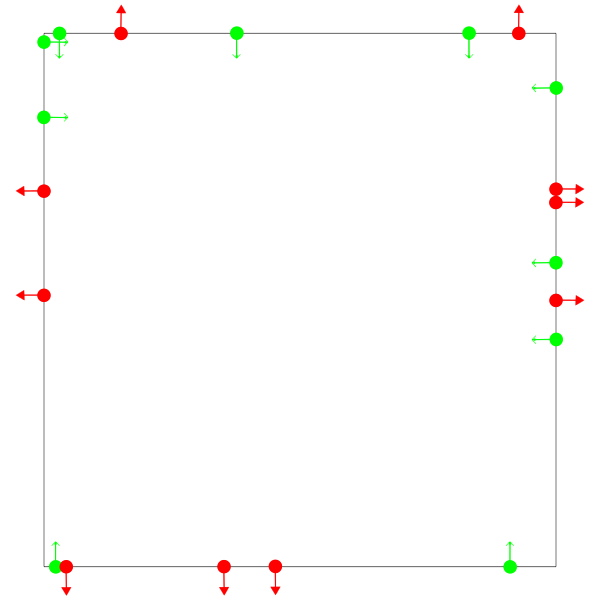
\includegraphics[width=\linewidth]{images/steps-input.png}
	 	\caption{Input}
	 \end{subfigure}
	 % 
	 \begin{subfigure}[b]{0.24\linewidth}
	 	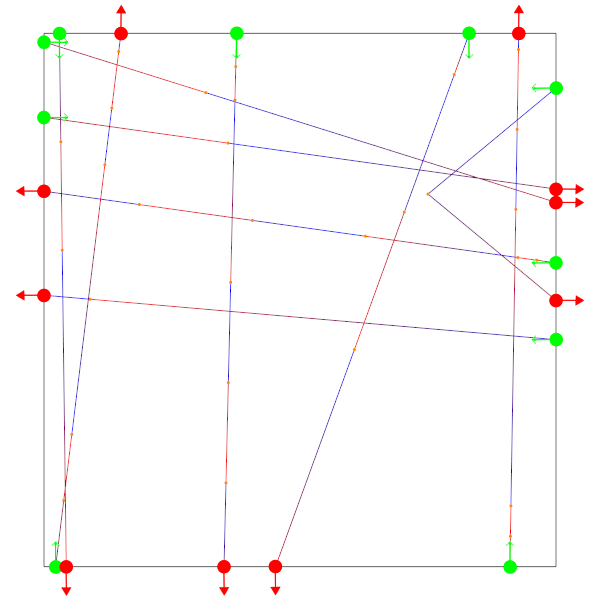
\includegraphics[width=\linewidth]{images/steps-connected.png}
	 	\caption{Connected}
	 \end{subfigure}
	 %
	 \begin{subfigure}[b]{0.24\linewidth}
	 	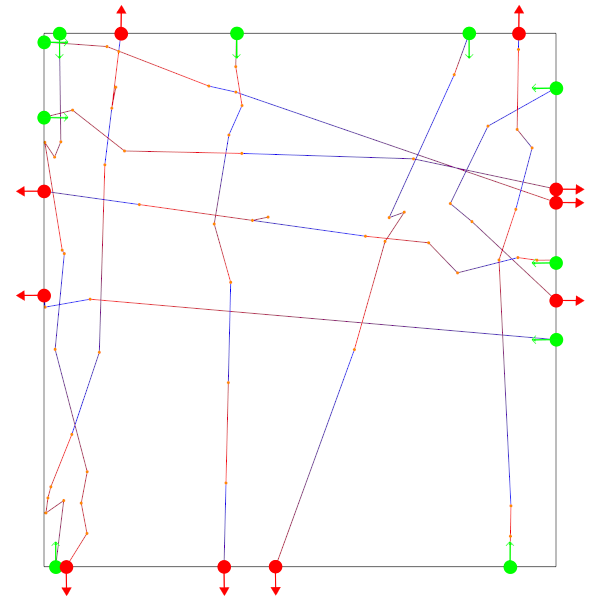
\includegraphics[width=\linewidth]{images/steps-collisionFree.png}
	 	\caption{Collision Free}
	 \end{subfigure}
	 %
	 \begin{subfigure}[b]{0.24\linewidth}
	 	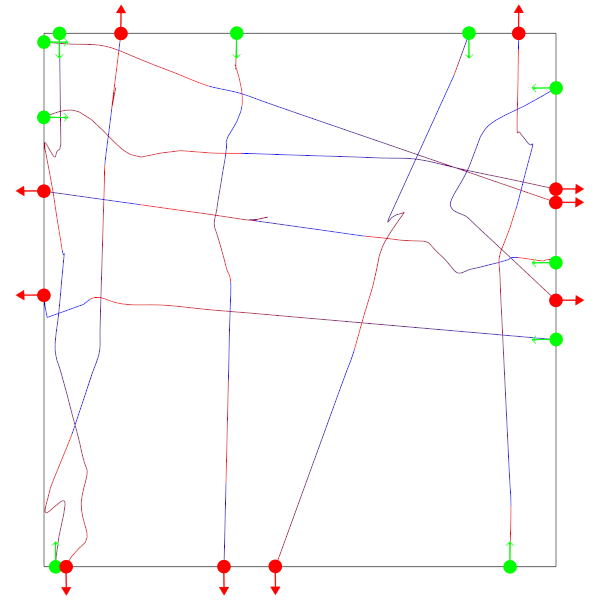
\includegraphics[width=\linewidth]{images/steps-smoothed.png}
	 	\caption{Smoothed Out}
	 \end{subfigure}
	 \caption{\textbf{Method example}
	 			The proposed method starts from
	 			(a) a set of control points in the boundaries of an empty patch,
	 			(b) interconnects them in an optimal way,
	 			(c) resolves any temporal collisions and finally
	 			(d) smooths the trajectories.
	 }
 \label{fig:res:steps}
\end{figure*}
%%----------------------------------------------------------------
%% Figure: Steps
%%----------------------------------------------------------------

\textbf{Adaptability to control point placement}
This method is able to adjust to the placement of the control points (Figure~\ref{fig:res:adapt-cp-placement}) aiming at the same time for good space coverage over the period of the patch.


\begin{figure*}[t]
 \centering
 \begin{subfigure}[b]{0.24\linewidth}
 	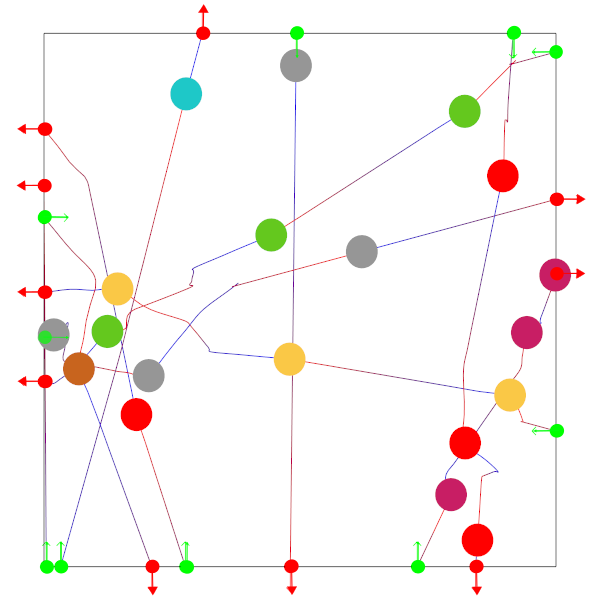
\includegraphics[width=\linewidth]{images/res-10-withAgents_1.png}
 	\caption{}
 \end{subfigure}
 % 
 \begin{subfigure}[b]{0.24\linewidth}
 	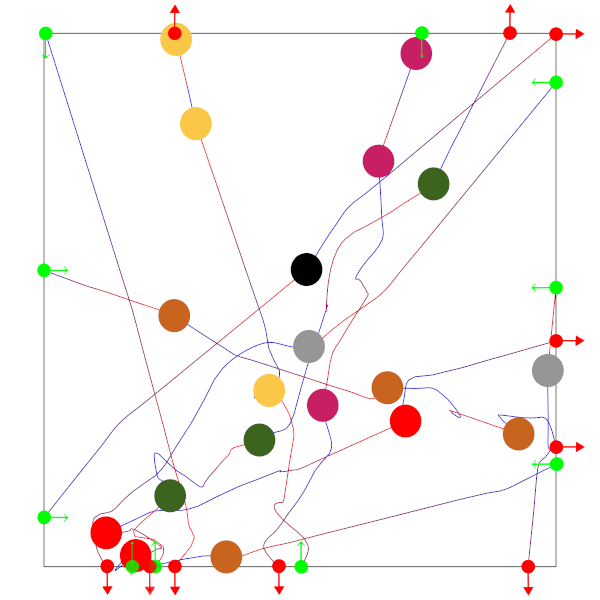
\includegraphics[width=\linewidth]{images/res-10-withAgents_2.png}
 	\caption{}
 \end{subfigure}
 %
 \begin{subfigure}[b]{0.24\linewidth}
 	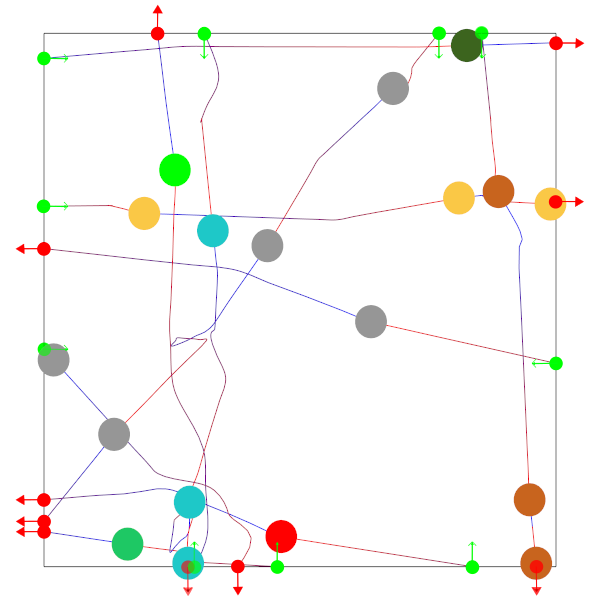
\includegraphics[width=\linewidth]{images/res-10-withAgents_3.png}
 	\caption{}
 \end{subfigure}
 %
 \begin{subfigure}[b]{0.24\linewidth}
 	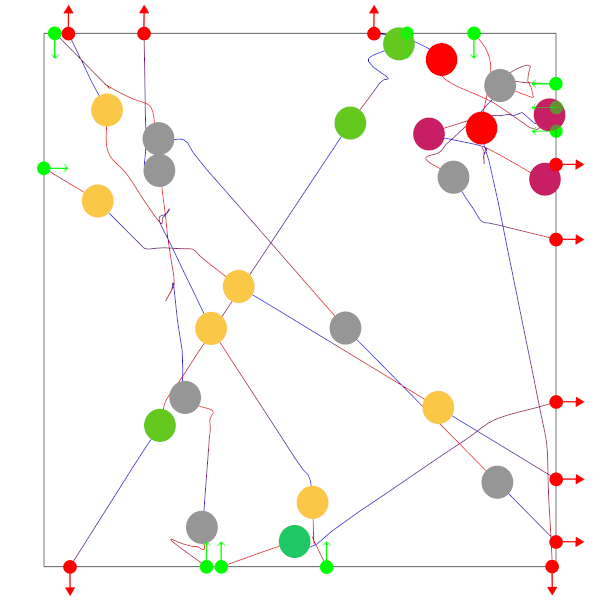
\includegraphics[width=\linewidth]{images/res-10-withAgents_4.png}
 	\caption{}
 \end{subfigure}
 \caption{
 	\textbf{Variance}
 	We demonstrate different results for the same number of initial spatio-temporal control points but different placement.
 	All the examples here consist of $10$ entry and $10$ exit control points.
%  	Several examples showing the final trajectories for 10 Entry/Exit Points
 }
 \label{fig:res:adapt-cp-placement}
\end{figure*}



\textbf{Adaptability to density}
The proposed method can adapt to different numbers of initial control points; i.e., it manages to generate smooth collision free trajectories for increasing larger numbers of trajectories (Figure~\ref{fig:res:inputs}).
Increasing the number of control points increases density and the time required for calculating these trajectories but recall that crowd patches are \emph{precomputed} and therefore during simulation time huge numbers of moving agents can be simulated at limited cost.
Again, trajectories aim to cover the patch's space.



%%----------------------------------------------------------------
%% Figure: Adaptability
%%----------------------------------------------------------------
\begin{figure*}[t]
	\centering
	%
	\begin{subfigure}[b]{0.24\linewidth}
		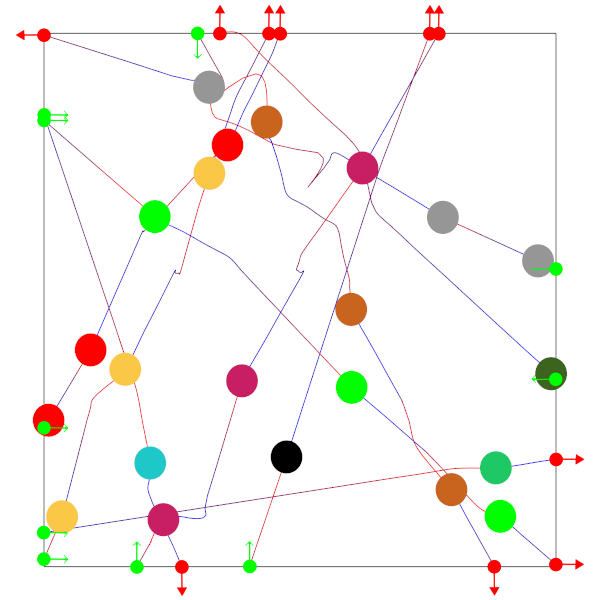
\includegraphics[width=\linewidth]{images/res-10-entry-exit.png}
		\caption{10 Entry/Exit Points}
	 \end{subfigure}
	%
	 \begin{subfigure}[b]{0.24\linewidth}
		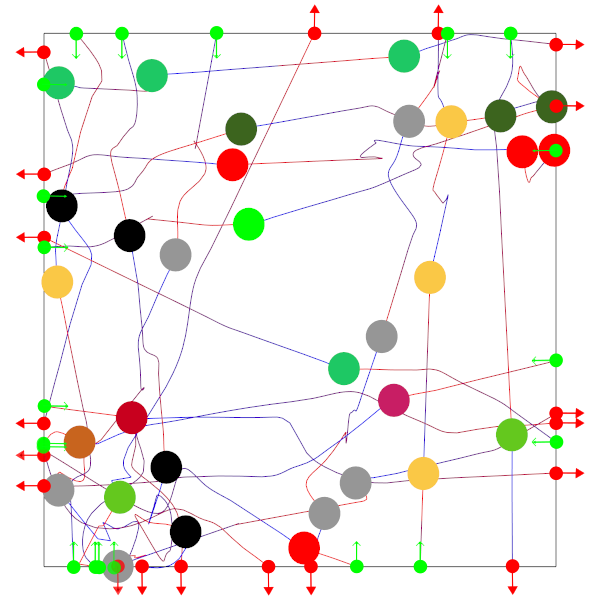
\includegraphics[width=\linewidth]{images/res-20-entry-exit.png}
		\caption{20 Entry/Exit Points}
	 \end{subfigure}
	%
	 \begin{subfigure}[b]{0.24\linewidth}
		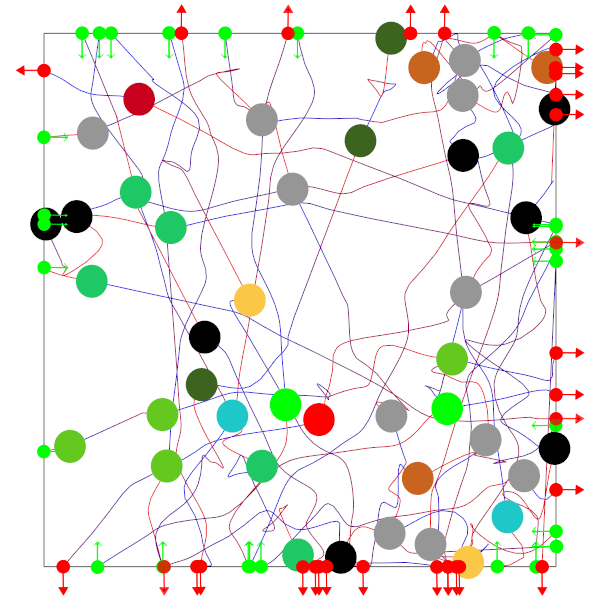
\includegraphics[width=\linewidth]{images/res-30-entry-exit.png}
		\caption{30 Entry/Exit Points}
	 \end{subfigure}
	%
	 \begin{subfigure}[b]{0.24\linewidth}
		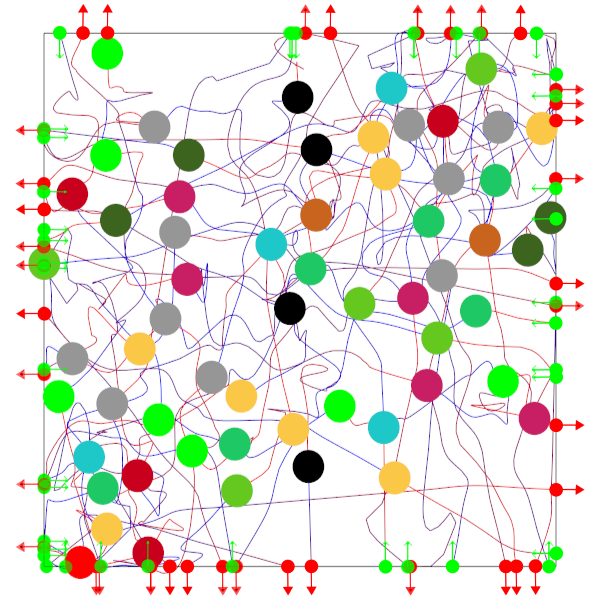
\includegraphics[width=\linewidth]{images/res-40-entry-exit.png}
		\caption{40 Entry/Exit Points}
	 \end{subfigure}
	%
	\caption{\textbf{Density Adaptability}
			The proposed method can generate collision free trajectories for many situations; from sparse to very dense.
			}
	\label{fig:res:inputs}
\end{figure*}
%%----------------------------------------------------------------
%% Figure: Adaptability to density
%%----------------------------------------------------------------


\textbf{Collision Anticipation}
In the original work~\cite{Yersin:2009} Helbing's social forces \cite{Helbing:2005} approach was used to handle collisions.
One problem with that approach is the lack of anticipation by agents; agents handle collisions late resulting in unnatural looking trajectories even for simple scenarios such as the one in Figure~\ref{fig:res:helbing} whereas the proposed approach emulates better anticipatory behaviour.

%%----------------------------------------------------------------
%% Figure: Collision Anticipation
%%----------------------------------------------------------------
\begin{figure}[t]
	\centering
	%
	\begin{subfigure}[b]{0.49\linewidth}
	 \centering
		\includegraphics[width=\linewidth]{images/res-helbing-crossing.png}
		\caption{Helbing}
	 \end{subfigure}
	%
	\begin{subfigure}[b]{0.49\linewidth}
	 \centering
		\includegraphics[width=\linewidth]{images/res-iter-crossing.png}
		\caption{Iterative}
	 \end{subfigure}
	% 
	\caption{
		\textbf{Collision Anticipation}
		(a) Using the approach described in \cite{Yersin:2009} trajectories lack anticipation as they suddenly curve when collisions are near whereas
		(b) the proposed method generates trajectories with higher anticipation resulting in gradually changing direction.
% 		The proposed method manages to generate trajectories with better anticipatory behaviour to \cite{Yersin:2009}
% 		A comparison between both methods, shows the improvement in terms of anticipating a collision. (a) shows little anticipation, it modifies its trajectory until it is about to collide, whereas (b) starts modifying its trajectory gradually from the beginning.
		}
	\label{fig:res:helbing}
%%----------------------------------------------------------------
%% Figure: Collision Anticipation
%%----------------------------------------------------------------
\end{figure}



%In Figure~\ref{fig:res:steps} we have a diagram showing the patch in various steps of our algorithm.
% Next we show the final curved trajectories with various sized input.
% Lastly we show some performance tests.We found that our algorithm created trajectories that were free of collisions and produced smooth motion. In Figure~\ref{fig:res:steps} we have a diagram showing the patch in various steps of our algorithm. Next we show the final curved trajectories with various sized input. Lastly we show some performance tests.












\section{Discussion}
\label{sec:discussion}

\textbf{Convergence}
The convergence of this algorithm, depends mostly on number of agents required in the virtual scene; large numbers of agents lead to long convergence time as well as the possibility the algorithm will not converge and the patch generation will fail.
Convergence failure can occur if at least two boundary control points are closer to the minimum allowed threshold $\alpha$ (Section~\ref{sec:method:remove-collisions}) at the same exact moment in time; this is by definition a convergence failure since \emph{boundary control points cannot be moved}.
If on the other hand, the boundary control points differ slightly in time, the algorithm will converge but with a high probability of generating agents with unrealistic speeds.

% There is an important limitation to be noted. 
% 
% A problem arises when two boundary control points that are closer than our collision threshold. If the points are also at exactly the same time the algorithm will not converge, since the only way to remove this collision is to move the boundary control points (which is forbidden). If the boundary control points are close in time collisions can be avoided, but may require the agents to move at unrealistic speeds.s

 Furthermore, two control points near the corners may have a repulsion force that pushes one of them to go outside the patch's boundaries.
For these cases, two approaches can be taken; either ignore these two points or let one of the two points leave the bounds of the patch.
%  we have to either tell the algorithm to skip them (since there is no way to solve the collision) or let one of them go out of bounds.
In the current implementation the latter was employed due to its simplicity.
 
 This leads to one important conclusion; given bad input (i.e., patterns and their boundary control points) the algorithm will behave badly resulting into bad trajectories.
 Therefore, we are currently looking into approaches of generating patches that will guarantee well behaved trajectories (defining well behaved trajectories is also an interesting problem).

% There may be better ways to deal with these problems, but no matter what the algorithm for computing these trajectories is, if the input to the patch is bad, the trajectories will be bad. So in the future we will look at generating input to the patch that does not have these problems.

\textbf{Temporal modifications of control points}
In this paper, mostly spatial corrections to the trajectories of the agents are employed.
For some scenarios, moving control points in space might not be the best approach, since this could results in either agents moving with unnatural speeds or accelerations or to trajectories leaving the area of the patch as described in the previous paragraphs.
Collisions can be avoided if temporal displacement is applied to control points without any spatial modification and in essence accelerate (or decelerate) agents.
Obviously, this could resolve spatial issues such as out of boundary cases but care should be taken so that agents' velocities remain realistic.

% it could provoke the control point to try moving outside of the patch boundaries or make a huge change in the agent's speed.   

% Some collisions may be avoided just by changing the time in one of the two movable control points of a segment, thus making the agent move faster or slower without modifying the spatial trajectory. This would solve the problem of going out of the boundaries, but we have to be careful on how we change the time if we don't want to produce an unrealistic change in velocity.  We also have to be careful that trajectories can never go backwards in time. 


\textbf{Obstacles}
A patch can have static objects; i.e., obstacles.
Having a small number of obstacles is equivalent to defining a set of special agents that are not allowed to move.
Obviously, placement of these obstacles plays a significant role on the trajectory generation since boundary control points could be ``trapped'' or if a trajectory passes closely between two static obstacles it would end up in a position where the collision avoidance algorithm would not converge since a control point could end up oscillating between the obstacles.
One possible solution to that is grouping obstacles together as a bigger one with a cost on the free area that can be used by other trajectories.
Approaches to handle dense obstacles are currently being considered as alternatices to this approach and on the design of crowd patches.
Obstacle handling is still under development.

% Earlier in this paper, it is mentioned that a patch may have static agents, called obstacles. The way of incorporating obstacles is still being discussed. For a small number of obstacles, they can be considered as special agents that do not move. The problem that arises is that obstacles must be well placed. When a trajectory travels between two obstacles it can cause an infinite loop. The trajectory will oscillate between the obstacles, but the collision will never be resolved. A possible solution for this, may be grouping the obstacles that are close to one another into a bigger obstacle. However, this would quickly start occupying the area of the patch. For that reason, a better technique for dealing with a dense number of obstacles must be developed. s

\textbf{Evaluating the quality of motion}
One of the largest issues in any crowd simulation work is evaluating the quality of the generated behaviour.
Currently, this is done by visual inspection.
Several methods have been proposed to evaluate the quality of crowd motion in a quantitative approach that we plan on investigating as future work.
For example Singh \etal~\cite{Singh2009SteerBench} propose to evaluate quality based on the capability of a crowd simulation algorithm of accomplishing simple scenarios.
Lerner \etal~\cite{Lerner2010Context} and Guy \etal~\cite{Guy2012Statistical} take an alternative approach where the quality of a crowd simulator is compared to real-world data.

\section{Conclusions}
\label{sec:conclusions}

We present a novel technique for computing trajectories for use in crowd patches. 
We can take an empty patch and generate trajectories within that can represent human motion. Our technique produces smooth collision free motion. This algorithm is slow to converge, especially with larger groups. Furthermore while our approach produces collision free trajectories it is lacking in other aspects of human motion. For one, agents can reach unrealistic speeds. Additionally agents can have abnormal motion that is not true to human behavior. In the future we plan to implement a more global approach that looks at more than just the closest agent and incorporates speed into the calculations. We hope that this will provide faster convergence in high density situations as will as fixing motion artifacts.

\note{ -  reminder of contributions
 - comment on results and limitations
 - paths for future work.
}

\section*{Acknowledgements}
Who do we love so much we want to worship them?
 

\bibliographystyle{acmsiggraph}
\bibliography{Crowd_Patches}
\end{document}
